%*************************************************************************
%*************************************************************************
%*                                                                       *
%*                          PHYS 506 Formal Report                       *
%*                                                                       *
%*                              Sample Report                            *
%*                                                                       *
%*                                Author:                                *
%*                               Your Name                               *
%*                                                                       *
%*************************************************************************
%*************************************************************************
%*                                 Notes:                                *
%*                                                                       *
%*  - A dedicated notes section is useful when collaborating with        *
%*    group members.                                                     *
%*                                                                       *
%*************************************************************************

%*************************************************************************
%****************************** Preamble *********************************
%*************************************************************************

%----------------------- Specify Document Type ---------------------------
% For one-column format:
\documentclass[prX,nofootinbib,notitlepage]{revtex4-1}

% For two-column format (which usually looks more professional):
%\documentclass[twocolumn,prX,nofootinbib,notitlepage]{revtex4-1}

% Note: The revtex4-1 document class includes a variety of Physics Journal
% styles. The option prX is specifies the Physical Review X journal style.


%*************************** Load Packages *******************************
% Note: Package descriptions and usage documentation can be found online
% at https://ctan.org/. Just use the site's search bar to search for the
% package

%------------------ Extending default LaTeX Structures -------------------
\usepackage{enumerate}
\usepackage{float}
\usepackage{caption}
\usepackage{hyperref}
\usepackage{subfiles}

%------------------------ Symbology \& Math ------------------------------
\usepackage{amsmath, amsthm, amssymb, amsfonts}
\usepackage{mathrsfs}
\usepackage{array}

%--------------------------- Graphics ------------------------------------
\usepackage[dvips]{graphics}
\usepackage{graphicx}
\usepackage{color}


%*************************************************************************
%****************************** Body *************************************
%*************************************************************************
\begin{document}

%************************ Document Settings ******************************

%---------------------- Bibliography Settings ----------------------------
\bibliographystyle{plain}


%****************** Title Information \& Abstract ************************

%--------------------------- Title ---------------------------------------
\title{Measuring the Charge to Mass Ratio of an Electron through Magnetism}

%----------------------- Author Information ------------------------------
\author{Luke Abanilla}%
\author{Eben Quenneville}
\author{Augustus Vigorito}
\affiliation{Department of Physics, University of New Hampshire,
Durham, NH 03824, USA}

%------------------------- Abstract --------------------------------------
\begin{abstract}
The constants of electric charge (\textit{e}) and the mass of an electron (\textit{$m_l$}) are extremely small quantities to measure. However, the ratio of these constants can be calculated by curving an electron beam using a magnetic field and measuring the radius of curvature. This is achieved using a device known as an “\textit{e}/\textit{$m_l$} of the electron apparatus.” The apparatus consists of a vacuum in a bulb with an anode that ionizes helium such that the path of electrons emitting from the electron gun in the bulb is visible. The curvature in the beam of electrons is caused by a pair of coils known as “Helmholtz coils” which induce a magnetic field by running a known current through the coils. Using this method, the team accurately measured the ratio of \textit{e}/\textit{$m_l$}.
\end{abstract}

\maketitle

%*************************** Introduction ********************************
\section{Introduction}
Measuring the mass to charge ratio of ions has been done in the past in the 19th century. This was measured first by J.J Thomson in 1897 using a cathode ray tube. This apparatus consisted of two metallic plates within a nearly evacuated glass tube. Within the glass tube, a very small amount of background gas remained. The cathode, which is the plate that has current passing through it, is heated and emits electrons that accelerate towards the anode, or positive terminal, of the cathode ray tube. The gas that is contained inside the glass tube scatters the electrons (i.e. ionizes the gas) and emits light, showing the path of the electrons as they reach the anode. By observing their motion, Thomson was able to measure and calculate the charge to mass ratio of an electron. This was repeated for different gases, and different metals for cathodes, each time producing the same value for the charge to mass ratio. From this, Thomson concluded that these particles he was observing had some negative charge and has a mass that was about 2000 times smaller than the lightest atom eventually naming them “corpuscles” which is now known as electrons. For this lab, the team will be following a similar process using a more sophisticated apparatus for measuring the path of the electrons.

%********************** Theoretical Background ***************************
\section{Theoretical Background} \label{Theoretical Background}

The charge and mass of an electron are incredibly important physical constants that appear throughout all of physics, from quantum mechanics to electromagnetism. Measuring the mass or charge of a single electron, however, is a very difficult task. Few of our instruments are capable of such a fine level of detail. A much easier task is to measure the ratio between the charge and mass. To do so, we need to find a method using information we already know. One way to do this is by using the Lorentz Force:
\begin{equation}
\vec{F} = q\vec{v} \times \vec{B}
\end{equation}
where $\vec{F}$ is the force that a charge $q$ moving at a velocity $\vec{v}$ feels due to a magnetic field $\vec{B}$. The apparatus uses the Lorentz force to deflect the electron into uniform circular motion at a measurable radius $r$. There are still multiple values in this equation that need to be experimentally found. However, it is easier to measure force, velocity, and magnetic field than the very small charge of the electron. We determine these other values by using a combination of equations. To begin, we can derive the strength of the magnetic field due to the apparatus by applying the Biot-Savart law. Consider a circular loop of current of some known radius $R$ centered at the origin with $N$ coils. By the Biot-Savart Law, the magnetic field at a distance $x$ from the origin is given by
\begin{equation}
\vec{B} = \frac{\mu_{0} I}{4 \pi ||\vec{r}||^{3} } \int\limits_{0}^{2\pi N}{d\vec{\ell} \times \vec{r}}
\end{equation}
where $\mu_0$ is the vacuum permeability constant, $I$ is the current flowing through the coil, and $\vec{r} = \vec{x} - \vec{R}$ is the vector from the point along the $x$-axis to some tiny arc of the coil $d\vec{\ell}$. Through careful algebraic manipulation and an application of the symmetry of the problem, it can be shown that 
\begin{equation}
\vec{B} = \frac{\mu_{0} I N R^{2}}{2(x^{2} + R^{2})^{3/2}} \hat{x}
\end{equation}
If we add a second current loop in series with the other one, centered at $x = R$, then by the Principle of Superposition the magnetic field at a distance $x$ along the axis is given as
\begin{equation}
B = \frac{\mu_{0} N I R^{2}}{2} \left( \frac{1}{(R^{2} + x^{2})^{3/2}} + \frac{1}{(R^{2} + (R-x)^{2})^{3/2}} \right)
\end{equation}
which, at a distance $x = R/2$, simplifies to 
\begin{equation} \label{Magnetic Field Equation}
B = \left(\frac{4}{5}\right)^{3/2} \frac{\mu_{0} N I}{R}
\end{equation}
with uncertainty
\begin{equation} \label{Magnetic Field Uncertainty}
\delta B = \sqrt{\left(\frac{4}{5}\right)^{3} \left(\frac{\mu_{0} N }{R}\right)^{2} (\delta I)^{2} + \left(\frac{4}{5}\right)^{3} \left(\frac{- \mu_{0} N I}{R^{2}}\right)^{2} (\delta R)^{2}} 
\end{equation}
Now, to find the velocity, we use a conservation of energy approach. The apparatus applies an accelerating voltage of $V$ to the charge $q$, which, assuming that the electrons begin at rest, is converted into kinetic energy as
\begin{equation}
qV = \frac{1}{2} m_{e}v^{2} \implies v = \sqrt{\frac{2qV}{m_{e}}}
\end{equation}
This velocity vector is perpendicular to the magnetic field by construction of the apparatus. For uniform circular motion, $F = mv^{2}/R$, so
\begin{equation} \label{Charge to Mass Equation}
qvB = \frac{m_{e} v^2 }{r} \implies \frac{q}{m_e} = \frac{2V}{r^2 B^2}
\end{equation}
with uncertainty 
\begin{equation} \label{Charge to Mass Uncertainty}
\delta (e/m_e) = \frac{2}{r^2 B^2} \sqrt{\delta V^2 + \frac{4}{r^2 }\delta r^2 + \frac{4}{B^2 } \delta B^2}
\end{equation}
where $r$ is the radius of the circular motion. In order to experimentally determine the ratio of charge to mass, we need to gather data about voltage, magnetic field, and the radius of circular motion. The techniques used to find this data are described below.


%*********************** Experimental Methods ****************************
\section{Experimental Methodology}

\begin{figure}[ht]
        \centering
        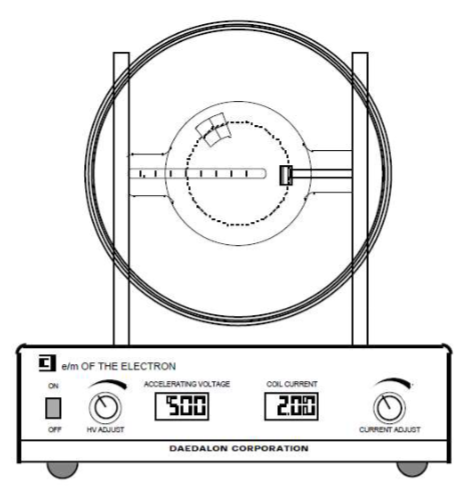
\includegraphics[width=0.5\linewidth]{exp 2 apparatus figure.png}
        \caption{\textit{e}/\textit{$m_l$} of the Electron Apparatus. Credit: \cite{PHYS506}.}
        \label{fig:apparatus}
\end{figure}

The apparatus (\ref{fig:apparatus}) consists of three internal power supplies, each of which provide power to the anode, current to the coils, and accelerating voltage for the electron beam. Externally, there are two large coils (depicted as a circle in \ref{fig:apparatus}). We measured, using a simple ruler, the inner and outer diameter of both coils. We assumed them to have the same diameter, and used the average (with appropriate uncertainty) as the diameter for our calculations. Power to the anode, or filament, is fixed while the panel controls vary the potential for the electron beam and the current to the coils. These values are measured by digital meters making it simpler to determine the forces acting on the electron beam. Within the bulb is an internal scale that measures the diameter of the path of the electrons in centimeters. Also included in the bulb is helium gas which fluoresces when hit by the moving electrons allowing for a much clearer view of the electron beam and better measurement. Additionally, at the end of the circular path of the electrons there is an electrode that absorbs the electrons after their path has been traced making measurements more accurate. 

\begin{figure}[h!]
    \centering
    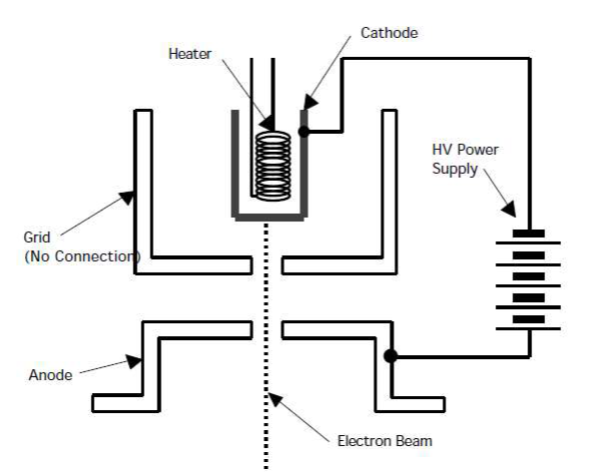
\includegraphics[width=0.5\linewidth]{exp 2 electron gun figure.png}
    \caption{Electron Gun Diagram. Credit: \cite{PHYS506}.}
    \label{fig:gun_schematic}
\end{figure}

Internally within the apparatus is an electron gun as shown above (\ref{fig:gun_schematic}). At the top is a cathode which is connected to the negative terminal of the high voltage supply. This cathode is indirectly heated, emitting electrons some of which pass through a small aperture in the surrounding grid. An anode is connected to the bottom of the grid which accelerates the escaping electrons due to the potential difference between the cathode and the anode. Although most electrons hit the anode, some pass through forming the electron beam visible in the experiment. 

In experimenting, we collected four data sets. To gather each we fixed an accelerating potential and then varied the currents through the Helmholtz coils and therefore the strength of the deflecting magnetic field. We then used the internal scale to measure the diameter of the path of the electron beam, and recorded the data points accordingly. This collection of points offering insights into the radius given a velocity and magnetic field allows us to determine the ratio of the charges, as described in the following section.


%---------- Sample Code for a Figure ----------
% \begin{figure}[h!]
% \centering
% \includegraphics[scale=0.55]{figure.jpg}
% \caption{A sample figure.}
% \label{fig:sampleFigure}
% \end{figure}
% Note: If your figure is not referenced anywhere in your document body,
% then you should not include that figure.

%************************ Results \& Analysis ****************************
\section{Results \& Analysis}

\begin{table}[h]
\begin{tabular}{|c|c|}
\hline
\textbf{Inner Diameter}~ $D_\text{int}$ ~\textbf{(cm)} & \textbf{Outer Diameter}~$D_\text{ext}$~\textbf{(cm)} \\\hline
28.5 & 30.5 \\\hline
28.5 & 30.8 \\\hline
28.5 & 30.9 \\\hline
28.5 & 30.9 \\\hline
28.5 & 30.7 \\\hline
\end{tabular}
\caption{Inner and Outer Diameter Measurements of the Helmholtz Coils}
\label{table:DiameterTable}
\end{table}

To proceed with the calculations described in \ref{Theoretical Background}, we began by calculating the radius of the Helmholtz Coils. The raw data is displayed in \ref{table:DiameterTable}. The best guess for the diameter is given as the average diameter, $\frac{\sum D_\text{int} + \sum D_\text{ext}}{N} = 29.63~\text{cm}$. The ruler we used to measure the diameter had a type-B uncertainty of $0.05~\text{cm}$, and the type-A uncertainty is given as $\delta D_{A} = \sqrt{\left(\frac{1}{N-1} \sum\limits_{i=1}^{N} (x_{i} - x_{\text{best}})^{2}\right)} = 0.075 ~\text{cm}$. Combining these results, our Helmholtz coil radius is
$$
R \pm \delta R = 14.8 \pm 0.1 ~\text{cm}
$$

We gathered current, radius, and voltage data experimentally. With that and our Helmholtz radius, we can apply our derivation of the magnetic field (\ref{Magnetic Field Equation}, \ref{Charge to Mass Uncertainty}) to calculate the strength and uncertainty of the magnetic field. The results of these calculations, with error bars, are displayed in \ref{fig:mag_field_data}. 

\begin{figure}[ht]
        \centering
        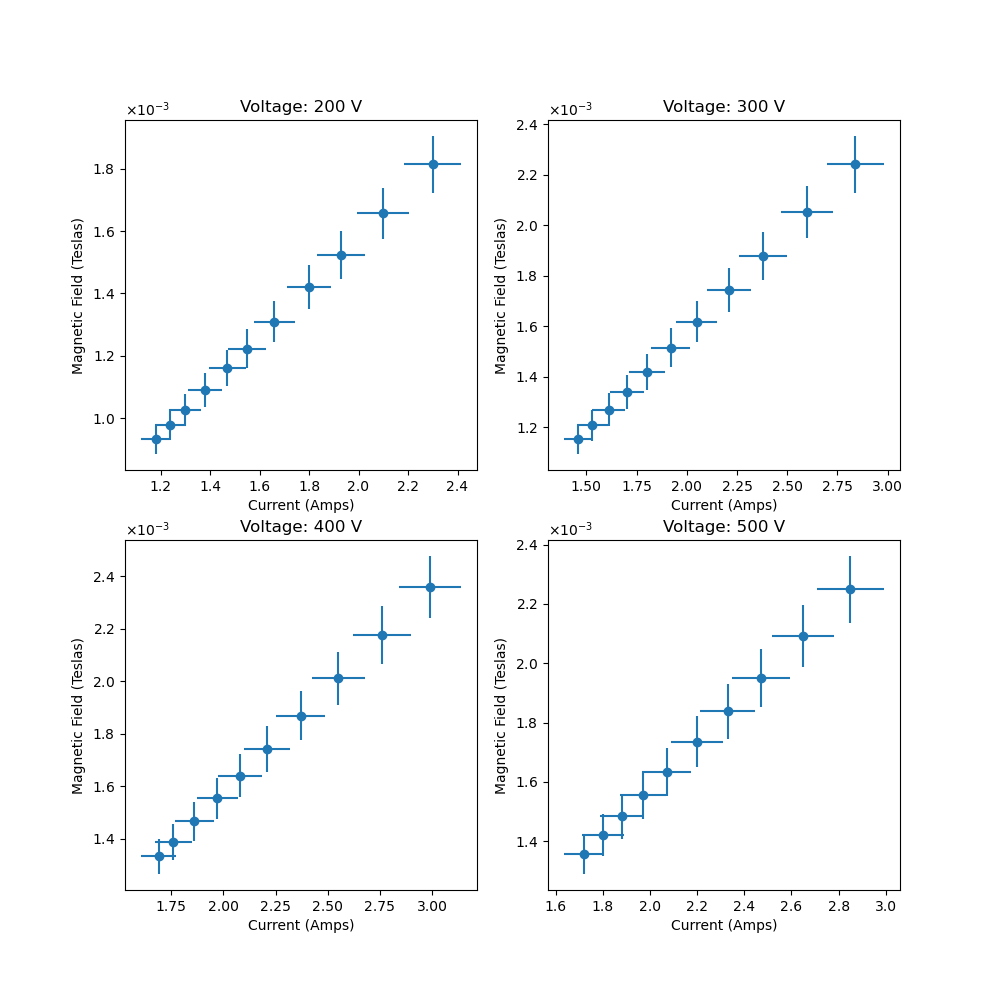
\includegraphics[width=0.75\linewidth]{MagneticField_vs_Current.png}
        \caption{Magnetic Field vs Current Data for Different Accelerating Voltages}
        \label{fig:mag_field_data}
\end{figure}

With the magnitude of $B$ calculated, we are able to use Equation \ref{Charge to Mass Equation} to determine the ratio of charge to mass for each current and voltage data point. We perform a weighted sum over all independent measurements to determine a best-guess value, as
\begin{equation}
(e/m_{e})_\text{best} = \frac{\sum\limits_{j=1}^{m}\left(w_{j}\left(\frac{e}{m_e}\right)_{j}\right)}{\sum\limits_{j=1}^{m} (w_{j})}
\end{equation}
where $w_{j} = \frac{1}{\delta(e/m_{e})^2}$. For the uncertainty in this summative measurement, we use
\begin{equation}
\delta(e/m_{e})_\text{total} = \frac{1}{\sqrt{\sum\limits_{j=1}^{m} w_{j}}}
\end{equation}
For the full derivation of these measurement calculations, refer to \cite{Lyons}. With these equations, we found the ratio of the charge to mass of an electron to be $\boxed{e/m_{e} = (-1.86 \pm 0.01) \times 10^{11} ~ \text{C/kg}}$. This result has a $5.75\%$ error from the agreed-upon NIST value of $(-1.75882001076 \pm 0.00000000053) \times 10^{11}~\text{C/kg}$ and an experimental disagreement. 

Many independent variables had to be measured in this experiment, yielding many compounding uncertainties. Of particular note was the uncertainty in voltage. We did not have a manual for the apparatus, so we assumed a Type-B uncertainty of $5\%$. This yields uncertainty on the order of $20~\text{V}$, which is very significant. One way to improve our result would be to find the manual and therefore the correct uncertainty in voltage. An additional improvement in experimental methods to make data-analysis more accurate would be to ensure that all data points are collected on the same interval as the dark characteristic data. This would make interpolating the zero points much easier and more accurate. An additional improvement that could be made is to use a compass to identify the Earth's magnetic field so that the Helmholtz coils can be positioned to minimize the effect of this external magnetic field. A more involved but equally valuable improvement would be performing the experiment in an electrostatically shielded environment to ensure the experimental data reflects only the intended system dynamics. We could also perform more repeated measurements under identical conditions to reduce random errors and improve the reliability of the final charge-to-mass ratio calculation.

%---------- Sample Code for a Small Data Table ----------
% \begin{table}[h!]
% \centering
% \begin{tabular}{|c||c|c|c|}
% \hline
% $a$ & $b$ & $c$ & $d$ \\
% \hline
% \hline
% $e$ & $f$ & $g$ & $h$ \\
% \hline
% $i$ & $j$ & $k$ & $l$ \\
% \hline
% \end{tabular}
% \caption{Sample data table.}
% \label{table:sampleDataTable}
% \end{table}
% Note: If your table is not referenced anywhere in your document body,
% then you should not include that table. Additionally, if the data set
% you want to present is very large, you should not use a table to
% present it. In this case, plotting your data appropriately is usually
% a more meaningful way to present the data.


%*************************** Conclusions *********************************
\section{Conclusions}
The charge to mass ratio of an electron can be calculated using the measurements of curving an electron beam through magnetism. Using the radius of curvature of the path the electrons follow, the team was able obtain an experimental value of $e/m_{e} = (-1.86 \pm 0.01) \times 10^{11} ~ \text{C/kg}$. The results, compared to the theoretical value provided by NIST is on the same order of magnitude with only a $5.75\%$ error, however, has an experimental disagreement due to the difference in uncertainty between the two values. This is due to the lack of an accurate value for the uncertainty of voltage in the apparatus. Despite this it is possible to measure the charge to mass ratio of an electron using magnetism and an understanding of Lorentz forces and Biot-Savart Law. 

%*************************** References **********************************
\begin{thebibliography}{99}

\section{References}

\bibitem{Lyons}
Lyons, L;
\textit{A Practical Guide to Data Analysis for Physical Science Students};
Cambridge Univ. Press; 1991.

% You should have several more references.
\bibitem{PHYS506}
Butbaia, Giorgi and Roberson, Matt;
\textit{PHYS506 - Experiment 2 Activity};
University of New Hampshire; 2024.

\end{thebibliography}

%*************************** Appendices **********************************
% \appendix
% \clearpage
% \section{Additional Information}\label{app:Additional}
% If there is more (data, discussion, derivations) you would like to present
% -- and that would be useful, relevant and informative to present -- that
% doesn't fit into the other sections, consider possibly adding an appendix.

\end{document}